%%% License: Creative Commons Attribution Share Alike 4.0 (see https://creativecommons.org/licenses/by-sa/4.0/)

\documentclass[english,10pt
%,handout
,aspectratio=169
]{beamer}
%%% License: Creative Commons Attribution Share Alike 4.0 (see https://creativecommons.org/licenses/by-sa/4.0/)

\DeclareGraphicsExtensions{.eps, .pdf,.png,.jpg,.mps,}
\usetheme{reMedian}
\usepackage{parskip}
\makeatother

\renewcommand{\baselinestretch}{1.1} 

\usepackage{amsmath, amssymb, amsfonts, amsthm}
\usepackage{enumerate}
%\usepackage{enumitem}
\usepackage{hyperref}
\usepackage{url}
\usepackage{bbm}
\usepackage{color}

\usepackage{tikz}
\usepackage{tikzscale}
\newcommand*\circled[1]{\tikz[baseline=(char.base)]{
		\node[shape=circle,draw, inner sep=-20pt] (char) {#1};}}
\usetikzlibrary{automata,positioning}
\usetikzlibrary{decorations.pathreplacing}
\usepackage{pgfplots}
\usepgfplotslibrary{fillbetween}
\usepackage{graphicx}

\usepackage{setspace}
\thinmuskip=1mu
\medmuskip=1mu 
\thickmuskip=1mu 


\usecolortheme{default}
\usepackage{verbatim}
\usepackage[normalem]{ulem}

\usepackage{apptools}
\AtAppendix{
	\setbeamertemplate{frame numbering}[none]
}
\usepackage{natbib}


% red strikeout
\newcommand\soutred{\bgroup\markoverwith
	{\textcolor{red}{\rule[0.55ex]{2pt}{0.8pt}}}\ULon}



% To use LyX frames from old version:
\def\lyxframeend{} % In case there is a superfluous frame end
\long\def\lyxframe#1{\@lyxframe#1\@lyxframestop}%
\def\@lyxframe{\@ifnextchar<{\@@lyxframe}{\@@lyxframe<*>}}%
\def\@@lyxframe<#1>{\@ifnextchar[{\@@@lyxframe<#1>}{\@@@lyxframe<#1>[]}}
\def\@@@lyxframe<#1>[{\@ifnextchar<{\@@@@@lyxframe<#1>[}{\@@@@lyxframe<#1>[<*>][}}
\def\@@@@@lyxframe<#1>[#2]{\@ifnextchar[{\@@@@lyxframe<#1>[#2]}{\@@@@lyxframe<#1>[#2][]}}
\long\def\@@@@lyxframe<#1>[#2][#3]#4\@lyxframestop#5\lyxframeend{%
	\frame<#1>[#2][#3]{\frametitle{#4}#5}}


\title{Mechanism Design}

\subtitle{0: Introduction}

\author{Egor Starkov}

\date{K{\o}benhavns Unversitet \\
	Fall 2020}


\begin{document}
	\AtBeginSection[]{
		\frame<beamer>{
			\frametitle{This slide deck:}
			\tableofcontents[currentsection,currentsubsection]
	}}
	\frame[plain]{\titlepage}


\section{What is mechanism design?}

\begin{frame}{What is Game Theory?}
\begin{center}
	Economic agents interact with each other.
	\pause
	
	$\Downarrow$
	
	What is the outcome? 
	
	How is it shaped by environment?
\end{center}
\end{frame}


\begin{frame}{What is Mechanism Design?}
\begin{center}
	\pause[2] 
	How to shape the environment to achieve it?
	
	$\Uparrow$
	
	\pause[1]
	There is some desirable outcome.
\end{center}
\end{frame}


\begin{frame}{MD Problem: Private Information}
\begin{itemize}
	\item MD problem is that of extracting private information from agents.
	
	\item MD does not really deal with inducing particular actions from agents -- because it designs the actions...
\end{itemize}
\end{frame}


\begin{frame}{MD Problem: Information Example}
\begin{exampleblock}{Not MD question\only<3>{ (?)}:}
	\begin{itemize}
		\item How should the employer \alert<1>{make people work}?
		\item Desired outcome: everyone works.
		\item Solution: \structure<1>{fire} anyone who doesn't work. Trivial!
	\end{itemize}
\end{exampleblock}
\pause
\begin{exampleblock}{MD question\only<3>{ (?)}:}
	\begin{itemize}
		\item How should the employer \alert<2>{make skilled people work harder}?
		\item Workers can pretend to be low-skill.
		\item Solution: ...? pay more for hard work? how much more?
	\end{itemize}
\end{exampleblock}
\pause
\begin{itemize}
	\item The line is subtle and depends on who you ask.
	\item But we will mostly be thinking about \structure{information extraction} problems
\end{itemize}
\end{frame}


\begin{frame}{MD Problem: Summary}
\begin{itemize}
	\item Mechanism design problem is one of shaping the environment that agents operate in in order to achieve some desirable outcome
	\item Outcome often depends on agents' private information 
	
	$\Rightarrow$ MD problem is that of extracting information.
	
	and determining which exactly outcome must be implemented in a given instance
\end{itemize}
\end{frame}


\begin{frame}{This course}
	What can you expect?
	\begin{itemize}
		\item overview of main results over past 40 years
		\item not that much from the frontier
		\item plenty of math! (brace yourselves)
		\item intuition and economics behind the models
		\item models are abstract but are applicable to a \textbf{lot of} areas (industrial organization, political economy, taxation, auctions\ldots{})
		\item see course description for more details on what exactly you learn
	\end{itemize}
\end{frame}


%\begin{frame}{This course}
%What is expected from you?
%\begin{itemize}
%	\item revise your math/game theory if necessary
%	\begin{itemize}
%		\item See a note on absalon for important topics.
%	\end{itemize}
%	\item a little bit of participation in the lecture
%	\item exercises (not handed in) between lectures
%	\item one week take home midterm assignment (groups allowed and recommended)
%	\item 24 hours take home exam (individual)
%\end{itemize}
%\end{frame}





\section{Logistics}

\begin{frame}{Hi}
\begin{itemize}
	\item Egor Starkov
	\item \texttt{egor.starkov@econ.ku.dk} or absalon inbox
	\item Research interests: information economics, dynamic games, communication
	\item Office: 26.1.13
	\item Office hours: Tuesdays 14:00-15:00.
\end{itemize}
\end{frame}


\begin{frame}{Logistics}
\begin{itemize}
	\item Weekly lectures (except Fall break -- week \#42, Oct 16)
	\begin{itemize}
		\item Fri, 12:00-15:00, CSS 2.2.02
	\end{itemize}
	
	\pause
	\item Mandatory midterm:
	\begin{itemize}
		\item one week take home (you can work in groups of up to 3 students)
		\item around fall break
		\item passing required to participate in the final exam
	\end{itemize}
	
	\item Final exam:
	\begin{itemize}
		\item 24hrs take home (individual, no groups)
		\item graded on usual scale
	\end{itemize}
\end{itemize}
\end{frame}


\begin{frame}{Covid-specific stuff}
	\begin{itemize}
		\item Rooms at half capacity, maintain 1m (2m?) distance at all times
		\item How do we do it?
		\begin{itemize}
			\item Mixed learning? (some students attend physically, some online, on a rotating basis)
			\item Go full online?
		\end{itemize}
	\end{itemize}
\end{frame}


\begin{frame}{Materials}
	\begin{itemize}
		\item This course is a compilation of many books, papers, courses; does not follow any single one too closely
		\item I expect lectures (sitting, listening, taking notes, reading slides afterwards) to be sufficient, material-wise, as long as you can fill in some (many) gaps
		\item Intended workflow: lectures $\to$ self catch-up $\to$ problems $\to$ questions
		\item I will be using the whiteboard, but also uploading slides to absalon. These serve as coarse lecture notes
		\begin{itemize}
			\item Slides will be on absalon by Friday mornings; updated versions with fixed typos (if required) after lectures
		\end{itemize}
		\item If you would like some external materials as well...
	\end{itemize}
\end{frame}


\begin{frame}{References}
	The following four references cover about 90\% of the class.
	\begin{itemize}
		\item textbooks:
		\begin{description}
			\item[B\"{o}rgers] Tilman B\"{o}rgers. An introduction to the theory of mechanism design. Oxford University Press, 2015.
			\item[RS] Roth \& Sotomayor. Two-Sided Matching: A Study in Game-Theoretic Modeling and Analysis. Cambridge: Cambridge University Press. 1990.
		\end{description}
		\item survey papers:
		\begin{description}
			\item[B\&V] Bergemann, Dirk, and Juuso Välimäki. ``Dynamic mechanism design: An introduction.'' Journal of Economic Literature 57.2 (2019): 235-74.
			\item[B\&M] Bergemann, Dirk, and Stephen Morris. ``Information design: A unified perspective.'' Journal of Economic Literature 57.1 (2019): 44-95. 
		\end{description}
	\end{itemize}
\end{frame}


\begin{frame}{References}
	alternative textbooks:
	\begin{description}
		\item[Diamantaras] Diamantaras, Cardamone, Campbell Deacle, and Delgado. A toolbox for economic design. Macmillan, 2009.
		\item[MWG] Mas-Colell,  Whinston, Green. Microeconomic theory. Oxford University Press, 1995. 
	\end{description}
\end{frame}


\begin{frame}{References}
	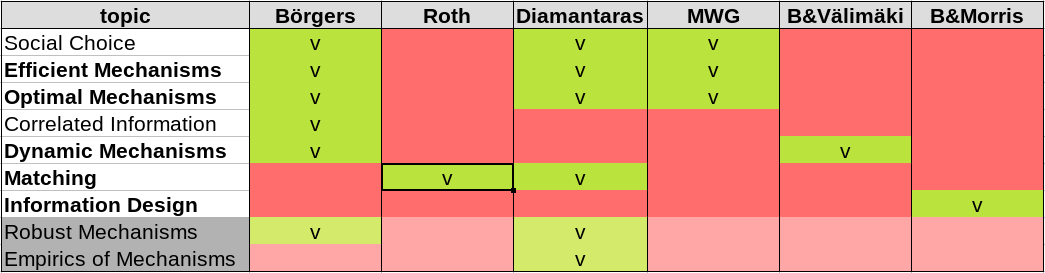
\includegraphics[width=\textwidth]{pics/L1/sources}
\end{frame}


\begin{frame}{References}
	In the end:
	\begin{itemize}
		\item I suggest getting B{\"o}rgers' textbook. It is not necessary, but might be useful.
		\item Diamantaras is a fine alternative.
		\item I do \textbf{not} recommend getting Roth \& Sotomayor textbook unless you are really interested in the topic. Promise the slides will be sufficient for that part of the class.
	\end{itemize}
\end{frame}


\begin{frame}{Related courses at KU}
\begin{itemize}
	\item Contract theory, Auctions
	\item Economics of organization, Corporate Finance
	\item Other courses in which applications of mechanism design appear:
	\begin{itemize}
		\item Public finance/Taxation
		\item Industrial organization
		\item Political economy
		\item Corporate finance
		\item Monetary
		\item Labor
		\item \ldots{}
	\end{itemize}
\end{itemize}
\end{frame}


\section{First taste}

\begin{frame}{First taste of what's to come}
	Let us now look at some of the ideas we will see in the rest of the course
	\begin{itemize}
		\item While using none of the methods!
		\item (To be clear: this following introduction is very informal and not representative of how you should solve exam problems)
	\end{itemize}
\end{frame}


\begin{frame}{The Trade Example}
	\begin{columns}
		\begin{column}{0.45\linewidth}
			In particular, consider the following situation:
			\begin{itemize}
				\item There is a \structure{seller} $i=0$ with one indivisible item, values it at zero
				\item There are \structure{two} potential \structure{buyers} $i=1,2$, who value the item at $\theta_i \in [0,1]$
				\item \alert{Valuations} $\theta_i$ are buyers' \alert{private} valuations, independent across $i$
			\end{itemize}
		\end{column}
		\begin{column}{0.55\linewidth}
			\includegraphics<handout:0>[scale=0.85]{pics/L1/negotiation}
		\end{column}
	\end{columns}
\end{frame}


\begin{frame}{Efficient Trade}
	\begin{block}{Question 1}
		How can we implement the \structure{efficient} outcome? (Buyer with the highest valuation gets the item)
	\end{block}
	\bigskip
	\begin{columns}[T]
		\begin{column}{0.4\linewidth}
			Objective relevant in, e.g., state auctions
			\begin{itemize}
				\item spectrum auctions
				\item land sale
				\item privatization 
				\item ...
			\end{itemize}
		\end{column}
		\begin{column}{0.55\linewidth}
			Possible formats:
			\pause
			\begin{itemize}
				\item Open bargaining (English/Dutch auction)
				\item Sealed-bid auction (first-price, second-price, all-pay)
				\item Contest (like APA, but winning probability smoothly depends on bid)
				\item all of the above can be static or dynamic
			\end{itemize}
			\pause
			Which are efficient?
		\end{column}
	\end{columns}
\end{frame}


\begin{frame}{Efficient Trade}
	\begin{itemize}
		\item ``implement an outcome'' = ``there exists an equilibrium which generates this outcome''
		\item Pretty much all mentioned formats have symmetric equilibria in monotone strategies
		\begin{itemize}
			\item (if bidders are symmetric)
			\pause
			\item Higher buyer's valuation $\Rightarrow$ higher bid $\Rightarrow$ highest valuation gets the item
		\end{itemize}
		\item So most symmetric auctions are efficient with symmetric bidders
		\item I want to focus on one particular format though...
	\end{itemize}
\end{frame}


\begin{frame}{Second-Price Auction}
	\textbf{Sealed-bid Second-price Auction}
	\begin{itemize}
		\item All players simultaneously submit bids $b_i$
		\item Highest bidder wins; pays second-highest bid.
	\end{itemize}
	\pause
	This auction is not only efficient in our simple story, but also
	\begin{itemize}
		\item has equilibrium in dominant strategies (rather than simple Bayes-Nash Eqm);
		\item remains efficient when other formats are not (e.g., asymmetric bidders);
		%\item yields the same expected revenue as any other efficient format.
	\end{itemize}
	Why does it all Just Work\texttrademark?
\end{frame}


\begin{frame}{Second-Price Auction: Equilibrium}
	It is easy to show that bidding own valuation is a weakly dominant strategy in SPA:
	\begin{itemize}
		\item suppose B1 values the item at $\theta_1$ and bids $b_1 > \theta_1$
		\begin{enumerate}
			\item if $b_2 < \theta_1$ then B1 wins and pays $b_2 < \theta_1$ (better than losing, same as bidding any $b_1 > b_2$)
			\item if $b_2 > b_1$ then B1 loses and pays nothing (better than winning by bidding $b_1 > b_2$)
			\item if $b_2 \in (\theta_1,b_1)$ then B1 wins and pays $b_2 > \theta_1$ (worse than losing because pays more than item is worth)
		\end{enumerate}
		\item The logic above applies to any $b_1 > \theta_1$. Bidding $b_1 \leq \theta_1$ dominates any $b_1 > \theta_1$ because avoids the loss in case 3 and yields same payoff in cases 1-2.
		\item Mirror logic applies to any $b_1 < \theta_1$:
		\begin{itemize}
			\item if $b_1 < b_2 < \theta_1$ then B1 loses, foregoing positive payoff from bidding $b_1 > b_2$ (e.g., $b_1 = \theta_1$).
			\item So this implies that bidding $b_1 \geq \theta_1$ dominates any $b_1 < \theta_1$.
		\end{itemize} 
		\item In the end, $b_1 = \theta_1$ is a weakly dominant strategy.
	\end{itemize}
\end{frame}


\begin{frame}{Second-Price Auction: Incentives}
	\begin{columns}
	\begin{column}{0.55\linewidth}
		What makes it tick?
		\medskip
		\begin{itemize}
			\item<2-> Bid affects in \structure{which states} of the world you get to win and at what price.
			\item<3-> Bid does not change the price you have to pay \structure{in a given state} (as long as you get the item)
			%\item<4-> ...%TODO: ...
		\end{itemize}
		\pause[4]
		\medskip
		These are powerful drivers of \alert{Incentive Compatibility}: agents not having incentives to pretend to have other valuations.
		
		IC is the main property that defines a working mechanism.
		
		(There is more to IC than the two features above)
	\end{column}
	\begin{column}{0.43\linewidth}
		\pause[0]
		\includegraphics<handout:0>[width=\textwidth]{pics/L1/multiverse}
		\begin{flushright}
			{\color{gray} \tiny Image credit: NASA, ESA, and G. Bacon (STScI)}
		\end{flushright}
	\end{column}
\end{columns}
\end{frame}


\begin{frame}{Wait a minute, Doc... are you telling me you built a mechanism?}
	We can use the same basic principles to implement any decision rule in general settings!
	\pause
	\begin{itemize}
		\item Say knowledge of \alert{state} of the world is dispersed among players
		\item Designer does not know state, wants to implement some state-dependent \alert{decision rule} (like the efficient one) using \alert{payments}
		\item Can do it via simple mechanism in which every player reports what they know to designer.
		\item Designer must devise such state-dependent payment schedule that:
		\begin{itemize}
			\item no player can lie and change their payment (in a given state) without also changing the decision. This is as before.
			\item payment levels are such that ...%TODO: ?
		\end{itemize}
		\item With \structure{efficient} decision rule, this is always possible. Otherwise possibility depends on rule and players' preferences.
	\end{itemize}
\end{frame}


\begin{frame}{Revenue Maximization}
	Back to the trade example.
	What if there is no specific decision rule to implement?
	\pause
	\begin{columns}[T]
		\begin{column}{0.55\linewidth}
			\begin{block}{Question 2}
				Which mechanism would maximize the seller's revenue?
			\end{block}
			\pause
			\begin{itemize}
				\item Now the seller/designer chooses the decision rule as well as payments.
				\item Recall all auction formats we mentioned. Which of them is more profitable?
				\pause
				\item None! All efficient mechanisms yield same revenue!
				\pause
				\item But what if... we violate efficiency?
			\end{itemize}
		\end{column}
		\begin{column}{0.4\linewidth}
			\centering
			\pause[2]
			\includegraphics<handout:0>[scale=0.6]{pics/L1/profit}
		\end{column}
	\end{columns}
\end{frame}


\begin{frame}{Revenue Maximization: Single Bidder}
	\begin{itemize}
		\item<+-> Idea is immediate if we look at the setting with \structure{one bidder} first.
		\item<+-> There are always gains from trade:
		\begin{itemize}
			\item bidder has positive valuation for the item;
			\item seller values it at zero;
			\item in any state there is some positive price at which a mutually beneficial trade can happen. (But this price depends on bidder's valuation)
		\end{itemize}
		\item<+-> Same insight applies as in Q1: bidder must not control price (conditional on trade).
		\begin{itemize}
			\item Given choice between ``buy thing at \$1'' and ``buy same thing at \$2'', who would choose the latter?
		\end{itemize}
		\item<+-> So price fixed. Efficient to trade always $\Rightarrow$ price would be zero! Not great for seller.
		\item<+-> Better to set positive price and exclude bidder with low valuation; to extract more from bidder with high valuation
	\end{itemize}
\end{frame}


\begin{frame}{Revenue Maximization: Many Bidders}
	Same applies with more than one bidder:
	\begin{block}{Key to revenue maximization}
		Exclude bidders with low valuations to extract more from bidders with high valuations.
	\end{block}
	\begin{itemize}
		\item In auctions: may be optimal to announce a positive reserve price
		\pause
		\item Kickstarter: maximize contributions by setting financing threshold and optional thresholds (?)
	\end{itemize}
\end{frame}


\begin{frame}{To be continued...}
	\begin{columns}
		\begin{column}{0.45\linewidth}
			This and much more we will look at in the remainder of the course.\\
			Stay tuned to learn more about designing all kinds of mechanisms!
		\end{column}
		\begin{column}{0.5\linewidth}
			\includegraphics<handout:0>[width=\textwidth]{pics/L1/design}
		\end{column}
	\end{columns}
\end{frame}


\end{document}